\documentclass[runningheads,a4paper]{./llncs2e/llncs}

\usepackage{graphicx}
\usepackage{caption}
\usepackage{subcaption}
\usepackage{amssymb}
\setcounter{tocdepth}{3}
%\usepackage{fixltx2e}
\usepackage{mathtools}
\usepackage{float}
\usepackage{wrapfig}
\usepackage[nolist,nohyperlinks]{acronym}
% Maintain images and tables within their respective sections
%\usepackage[section,subsection,subsubsection]{extraplaceins}
\usepackage{epstopdf}
\usepackage[utf8]{inputenc}
\usepackage{listings}
\usepackage[usenames,dvipsnames]{color}
\usepackage{url}
\usepackage{lipsum}

\setcounter{secnumdepth}{3}

%
% Change the margins
%
% \usepackage[margin=2.9cm]{geometry}

\begin{document}
\title{Procedural Generation}

\subtitle{City Modeling}
\author{Artur Alkaim}

\institute{Instituto Superior Técnico, Universidade de Lisboa
\path{arturalkaim@tecnico.ulisboa.pt}\\
\url{http://tecnico.ulisboa.pt/}}

\toctitle{Procedural Generation}
\tocauthor{Artur Alkaim}
\maketitle

\newenvironment{absolutelynopagebreak}
  {\par\nobreak\vfil\penalty0\vfilneg
   \vtop\bgroup}
  {\par\xdef\tpd{\the\prevdepth}\egroup
   \prevdepth=\tpd}

\lstdefinestyle{racket}{
  language=Lisp,
  basicstyle=\tt\small,
  columns=fullflexible,
  commentstyle=\color{Gray},
  keywordstyle=\color{Blue},
  identifierstyle=\color{Blue},
  stringstyle=\color{Green},
  numbers=left,
  numberstyle=\small\tt,
  frame=lines,
}

%!TEX root = ../report.tex

% 
% Abstract 
% 

\begin{abstract}

The existing graphic creation tools are geared for manual use. Unfortunately, the manual production of large amounts geometry is very time consuming. Procedural generation of these forms is one of the approaches which considerably speed up this process. This approach consists in the algorithmic construction of these forms and allows the creation of massive amounts of geometry very fast. As these tools were not made specifically for this type of use, favoring manual use, they do not have the high performance necessary for smooth use as it takes a long time since we run the program until you can see the result. This work proposes a solution for this performance problem, through the use of different techniques and technologies to accelerate the visualization of large amounts of geometry.


%The existing graphic creation tools are geared for manual use. Unfortunately, the manual production of large amounts of complex architectural forms is very time consuming. Procedural generation of these forms is one of the approaches which considerably speed up this process. This approach consists in the algorithmic construction of these forms through different techniques like shape grammars, L-Systems, etc. This project aims to explore this approach and apply it to the procedural modeling of cities by the development of a tool that, in connection with the Rosetta tool, will provide a new mean for the users to explore this approach. (\dots)

\end{abstract}
%!TEX root = ../report.tex

% 
% Keywords 
% 

\begin{keywords}

3D modeling, OpenGL, Generative Design, Procedural Generation, Shaders

\end{keywords}
%!TEX root = ../report.tex

% 
% Introduction
% 

\section{Introduction}

%General description of the problem and its context, current solutions, and road map of the project.

%This days designers and developers have available a large number of Computer Aided Design(CAD) tools to produce their models. This tools are getting more and more powerful and with more features available. The tradicional way of modeling where the user adds geometry one by one does not present performance issues about rendering. On the other hand it is being more and more common the concept of denerative design, that is a design method that is based on a programming approach which allows architects and designers to model large amounts of shapes with significantly less effort.

As technology evolves and people get new and more powerful devices, they want to take advantage of that and have more realistic\textbf{(powerful ?)} experiences with larger, more detailed and complex contents.
And this is observable in the graphic contents. With the recent extra high definition on screens and the computational power of the machines beating records, the graphic content have to follow up that characteristics in quantity as well as in quality. The issue is that the manual content generation takes a long work time from architects and designers to achieve this quality, thus implying high costs.

Graphic contents are mainly used for enterteinment, both in the gaming and movie industries, but it is also used in a lot more different areas. The fields of architecture and design, for instance, use this technique to experiment and model new designs, from small objects like a plate to buildings or even entire cities. So also in this field they face also the problems that raises from the modelling of really big sets of objects and forms manualy. \emph{This work focus on this problem of content creation for the fields of architecture and design.}

The obvious answer to this problem of manual content creation costs is to contract more architects or designers to each project to increase the production, but experience have shown that this solution is not scalable, that means that double the number of architects or designers working in a project will not double their overall productivity. Also this solution have a big impact on costs, that would take immediately out of the market new producers with less resources.

A solution for this problem is the use of generative design. That is a design method that is based on a programming approach which allows architects and designers to model complex shapes with significantly less effort. 

Although most computer-aided design (CAD) applications provide programming languages for generative design, programs written in these languages have very limited portability. This languages are not pedagogical and and are dificult to use even to experienced programmers, problems that create barriers to adherence to this approach by users that normally are not used to code.\cite{ramos_et_al:OASIcs:2014:4565}

There are several tools that aim to break down some of this barriers and facilitate the approximation of these individuals to programming. 

%There is a tool that aims to break down some of this barriers and facilitating the approximation of these individuals to programming. It is \textbf{Rosetta}, an extensible IDE based on \textbf{DrRacket} and target at architects and designers.\cite{lopes2011portable} The users specify their models in Rosetta that generates the geometry and transports all this data to the CAD tool that then moves the data to the GPU to graphics visualization. Rosetta works with various CAD tools because it also have interoperability as a special concern. 

With this rises the problem of performance because running this code is much faster than manual modeling, so the user is able to create massive amounts of geometry fast with tools like Rosetta and they usually have to wait a lot of time for all that geometry to be generated and then rendered for visualization. It takes a lot of time to generate this geometry but the communication and data transfer also have a significant role on this wait. This problem is more important in the development phase when the model is always changing and the user wants to see the effect of small changes immediately, if with each small change they have to wait a significant amount of time it have a significant impact for the work of the designers.

%There is an area of research that addresses this problem named \emph{Procedural Content Generation}, or \emph{Procedural Generation}. This have applications for example in the creation of large and/or complex scenarios for games and movies or the creation of models to use for simulation of cities. This examples involves the generation of large amounts of forms that would be impracticable with the manual approach to content creation.

This work is being developed in the context of Rosetta and proposes a solution to this problem. It does it by eliminating layers while trying to transfer the minimum possible data between layers. First we aim to get the geometry as fast as possible to the GPU, so since our goal is just visualization we jump the CAD layer. Another action is to reduce the amount of data that is transferred and it is achieved by transferring only a very concise description of the geometry that is generated by code running on the GPU. Also some techniques will be studied and applied to improve performance.




%FALAR DO FEEDBACK A DAR AO USER


 






 
%!TEX root = ../report.tex

% 
% Overview
% 

\section{Overview} % (fold)
\label{sec:overview}


This section will provide an overview of this topic.  Section~\ref{sec:related_work} will explore related work. Section~\ref{sec:objectives} will address the objectives for this thesis work. Section~\ref{sec:architecture} will describe the architecture of the proposed solution. Section~\ref{sec:evaluation} will explain how this solution will be evaluated and section~\ref{sec:conclusions} will conclude this work.

\subsection{Procedural Modeling} % (fold)
\label{sub:procedural_modeling}

\emph{Procedural Modeling} is the algorithmic generation of content instead of the usual manual creation of content. This can be applied in almost all forms of content, but is mostly used in the generation of graphic content, such as textures, geometry and animations, in which is included generative design. Procedural generation is also used for the generation of sound, with procedurally generated music and synthetic speech.

The key property of procedural generation is that it describes the data entities, such as textures, geometry, or sounds, in terms of a sequence of instructions rather than as a static block of data \cite{Kelly}. This allows the production of big volumes of detailed, high quality, graphic content without the costs, both in time and money, of manual content creation. Since it is based on procedures, it provides parametric control. Users can introduce in their programs as many useful parameters as they want, which allows them, for instance, to have different results from just one implementation by just changing some control values.
%!TEX root = ../report.tex

% 
% Objectives
% 

\section{Objectives}
\label{sec:objectives}

The world population has grown at a faster and faster pace, which is causing overcrowding and large migration flows. The problem is that most countries are not prepared to accommodate this people. 
To solve this problem that occurs in countries like China or the Emirates, new cities are being built  completely from scratch. An example of these cities is the city of Maasdar\footnote{\url{http://www.masdar.ae/en/masdar/detail/masdar-city-free-zone}} in Abu Dhabi. This city, designed by Foster and Partners, is currently being built in the desert and has an estimated cost between 18 and 19 billion US\$. Whoever is responsible for a project of this size can not afford to make any mistake.
To test all this factors it is necessary to create models, but in contrast to the relatively small size of a model of a single building, in this situations an entire city has to be modeled. Therefore requires generation and visualization of very large amounts of geometry.

The overall goal of this work is to build a GD tool that solves the performance problems that raise with the modeling and generation of large amounts of geometry. It should be an easy to use tool, with very high performance that will be focus on model visualization, removing features regarding interactive model manipulation.

It also should be able to support Immediate Feedback for much larger models than the current GD tools can handle. This system should also provide a significant amount of geometric primitives such as \emph{boxes}, \emph{cylinders} or \emph{spheres} that will allow users to model.

It will also provide a programming interface, that is how users will interact with the system. It should be simple and easy understand, yet broad and powerful to give the users freedom to create. This will be the visible part of the system together with the visualization window.

After, there is the \textbf{GPU communication} module that implement the functions provided. This module will generate the geometry description, create the windows and transfer the data to the GPU. This module will implement a set of techniques that will 

The \textbf{GPU pipeline} is where the geometry will be generated and is explained in Section~\ref{sub:modern_opengl}.


This work is being developed in the context of the Rosetta that is also a GD tool that helps architects and designers to develop their work procedurally. Rosetta is an extensible IDE based on \textbf{DrRacket} and built in Racket. 

In this context the module will act as a fast preview mode that allows the users to rapidly see the changes they make on their model during their creative process.

On the next section will be presented related works that have similar objectives.


%The world population has grown at a faster and faster pace, which is causing overcrowding and lack of resources in various locations of the globe. For example in the Emirates, the economic boom supported by the oil business is creating lots of work oportunities, thus thousands of people from everywere in the world are moving there. However the country was not prepared to accommodate the growing population currently living there. 
%To solve this problem of overpopulation that occurs there, and in other countries like China, new big cities are being built in the desert completely from scratch. An example of these cities is the city of Maasdar in Abu Dhabi. This city designed by Foster and Partners and currently being built in the desert and an estimated cost between $US\$18 and 19 billion$. Who is responsible for a project of this size can not afford to make a mistake in choosing the location or city setting.
%To test these factors is necessary to create models , only in contrast to the relatively small cost of creating manually using traditional techniques , model a single building with some variations , nestad situations have to be modeled an entire city and even variations additional. This  design phase is therefore very costly in time and effort required to enable them to obtain the best possible result.

%The objectives of this project are to study the existing approaches to Procedural Generation and provide a solutions to the kind of problems, like the new city in Abu Dabi stated above, through the implementation of mechanisms for procedural generation of architectural form, with application to the generation of large amounts of forms, such as of urban environments, buildings and ornaments efficiently and according to a particular architectural style models.

%With the large amount of very different techniques, explained in Section~\ref{sub:procedural_modelling_techniques}, one important part of this work is to know where to apply each techinque to obtain better results.

%!TEX root = ../report.tex

% 
% Related work
% 

\section{Related Work}
\label{sec:related_work}

As an active research field inside Computer Science, there is a lot of work being done in this area. In this section I give an overview of the related work that has been carried out on procedural generation of large amounts of geometry. Since the target audience of this work are architects and designers, most of the work that I present have the same target.

The main goal of this systems is to generate models that represent entire cities, that are large by definition. With this, they face some of the same problems I face so it is important to learn about their solutions.

%The related work section will highly volatile, and will mostly depend on your kind of thesis. Talk with your supervisor in order to know how to write this part. Don't take the following bullet points as a certain truth.


%!TEX root = ../../report.tex

\subsection{CityEngine \cite{Parish2001} \cite{Muller2006}}
\label{sub:cityengine}

CityEngine is a three-dimensional (3D) modeling software developed by Procedural Inc. (now part of the Esri R\&D Center). Specialized in the generation of 3D urban environments. With the procedural modeling approach, CityEngine enables the efficient creation of detailed and large-scale 3D city models with a lot of control from the user. This system applies the concept of Immediate Feedback by allowing the user to immediately see the results of each change. This is implemented through a set of sliders that are assigned to various indicators in the model that can be as high level as the \emph{size of the city} or as specific as the width of the windows or the number of floors in a building.

The following sections explain how CityEngine faces each of the steps in the generation of a city, such as road network generation or building modeling.

\begin{figure}[htbp]
  \centering
  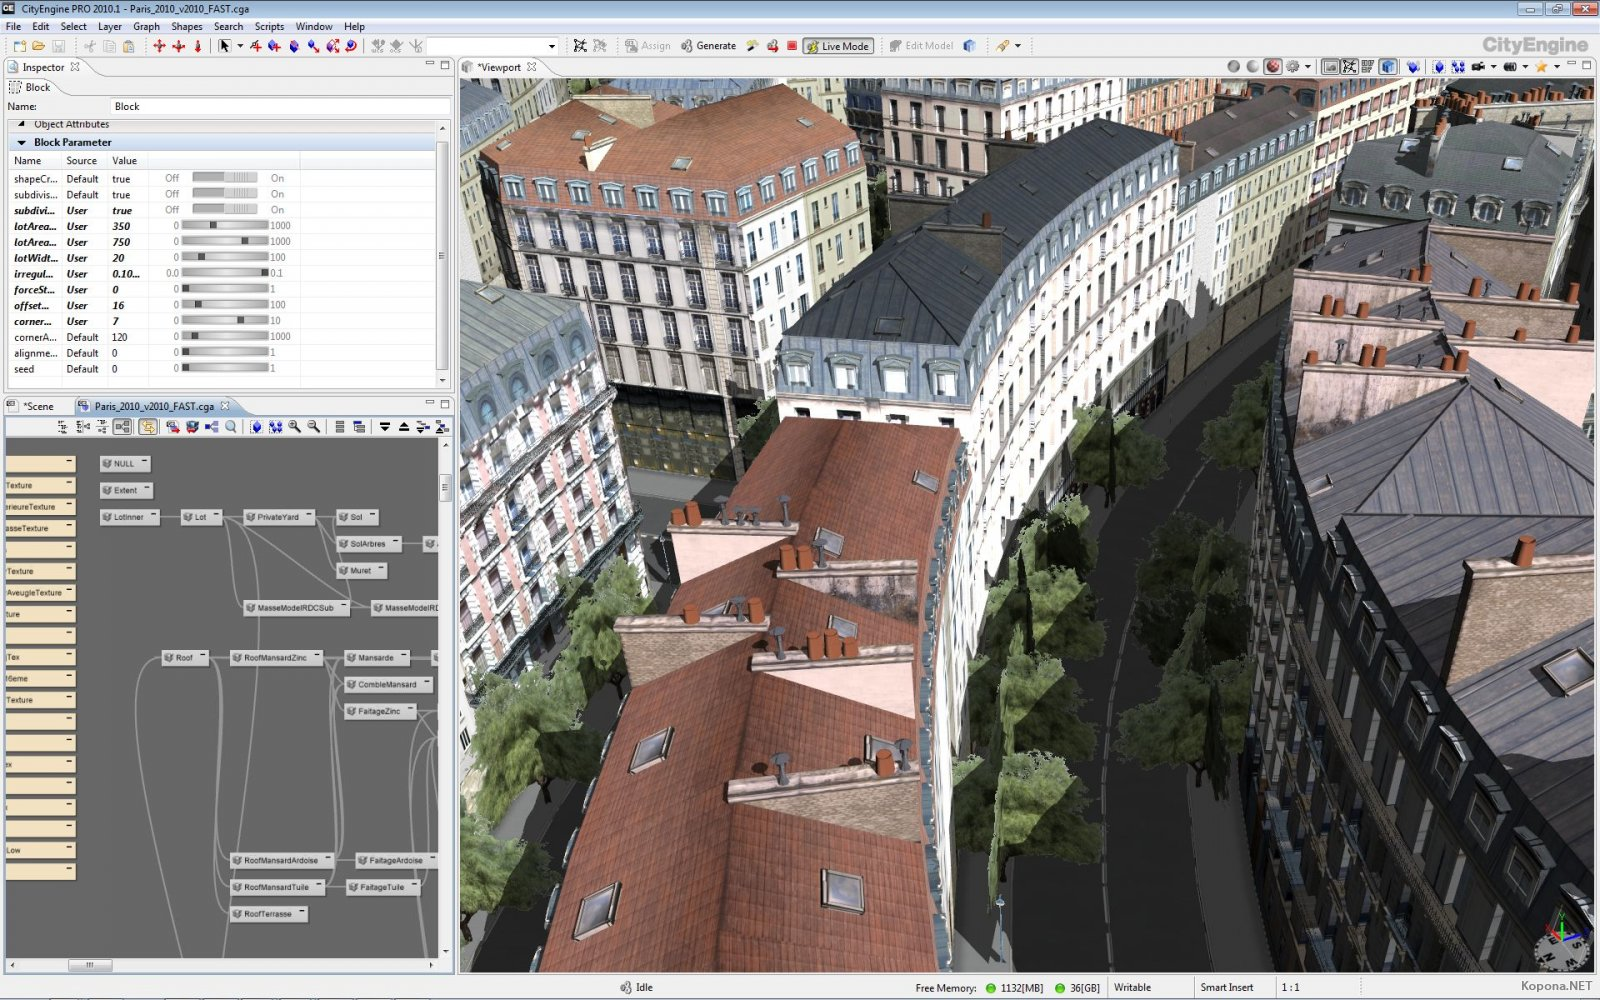
\includegraphics[width=\textwidth]{img/Procedural-Modeling-of-Cities/interface.jpg}
  \caption{City Engine Interface}
  \label{fig:CEinterface}
\end{figure}

\subsubsection{RoadNetwork} % (fold)
\label{ssub:roadnetwork1}


The first part to procedurally generate a city is to create a road network to become a backbone of the city and provide an overall structure. For that, CityEngine receives as input maps such as land-water boundaries and population
density. From that input a network of highways is created to connect the areas off high density population, and small roads connect to the highways.
This growth process continues until the average area of each lot is the desired one. The system have a default value, but it can be set by the user to a different one.

To implement this growth process, it uses an L-System (Section~\ref{ssub:l_systems}) that computes the road network.


\begin{figure}[htbp]
  \centering
  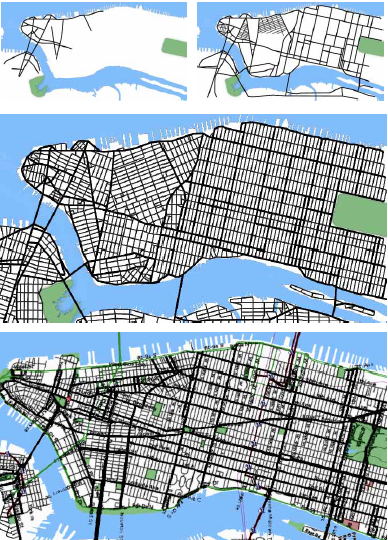
\includegraphics[width=0.5\textwidth]{img/Procedural-Modeling-of-Cities/Capturar.png}
  \caption{Road Map growth}
  \label{fig:city}
\end{figure}

The Figure~\ref{fig:city} shows the evolution of this process in a map of Manhattan. The first two pictures on the top shows the process in different phases during the process, the picture in the middle is the result of the process and the bottom line is the real map of Manhattan for comparison.

% subsubsection roadnetwork (end)Road Network

\subsubsection{Buildings} % (fold)
\label{ssub:buildings1}

To implement the generation of buildings, CGA was created, which is a shape grammar(Section~\ref{ssub:shape_grammars}) that was introduced in \cite{Parish2001}. It is defined as ``a novel shape grammar for the procedural modelling of CG architecture, produces building shells with high visual quality and geometric detail." To do so, this grammar uses a group of well defined production rules.

This tool allows the user to model buildings with an high control and in different ways. It can be done by text, writing production rules from a shape grammar or with a visual language similar Grasshopper 3D, that is nice for simple models but it is hard to work with more complex models, for instance, Figure~\ref{fig:CEinterface} shows a set of rules (bottom left), that is relatively small but is already difficult to follow the connections between rules.

\paragraph{Mass Modeling} % (fold)
\label{par:mass_modeling}
To model a building the first step is to create a mass model of the entire building by assembling basic shapes. With scaling, translation rotation and split applied to basic shapes namely I, L, H, U and T as shown in the Figure~\ref{fig:basic_shapes}.

\begin{figure}[htbp]
  \centering
  
\includegraphics[width=0.95\textwidth]{img/Procedural-Modeling-of-Cities/MassModeling2.png}
  \caption{Basic shapes}
  \label{fig:basic_shapes}
\end{figure}

% paragraph mass_modeling (end)

The next step is to add the roof, from a set of basic roof shapes or general L-Systems.

After that, with the application of the grammar rules in the created mass, it is possible to create complexity to the level that is desired, being able to produce highly complex buildings like the one in Figure~\ref{fig:CEnewbuilding}.


\begin{figure}[htbp]
  \centering
  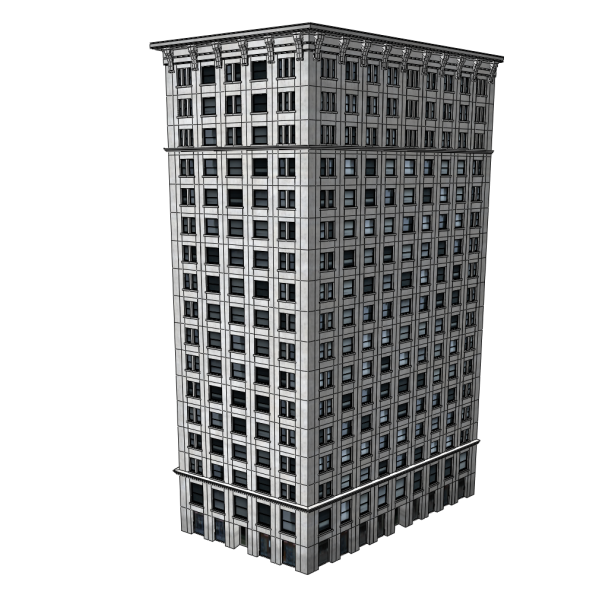
\includegraphics[width=0.8\textwidth]{img/Procedural-Modeling-of-Cities/building2.png}
  \caption{Complex building modeled with CGA}
  \label{fig:CEnewbuilding}
\end{figure}

% subsubsection buildings (end)

\subsubsection{Cities} % (fold)
\label{ssub:Cities1}

The result can be a city like Figure~\ref{fig:bigCity}, with approximately 26000 buildings.

\begin{figure}[htbp]
  \centering
  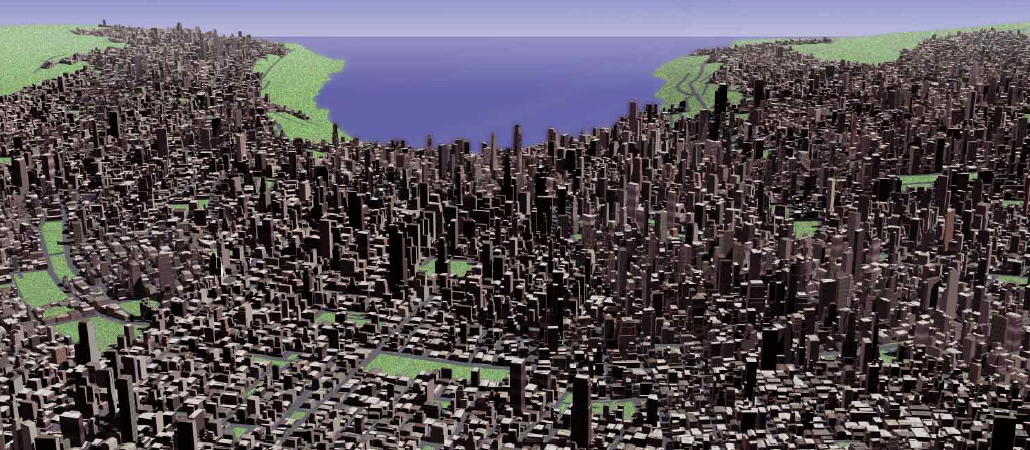
\includegraphics[width=0.95\textwidth]{img/Procedural-Modeling-of-Cities/City.png}
  \caption{City with approximately 26000 buildings.}
  \label{fig:bigCity}
\end{figure}

City Engine outputs can be imported by Maya\footnote{\url{http://www.autodesk.com/products/maya/overview}}, to achieve better results. Like the Figure~\ref{fig:cityMaya}, that represents a ‘virtual’ Manhattan.

\begin{figure}[htbp]
  \centering
  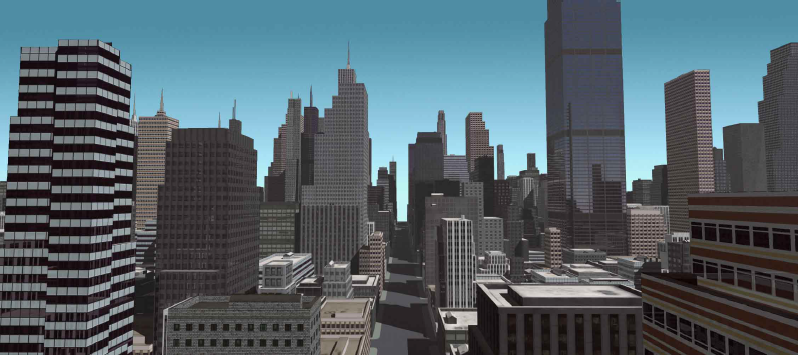
\includegraphics[width=0.95\textwidth]{img/Procedural-Modeling-of-Cities/City_Maya.png}
  \caption{City rendered with Maya.}
  \label{fig:cityMaya}
\end{figure}

% subsubsection subsubsection_name (end)

%!TEX root = ../../report.tex

\subsection{Undiscovered City} % (fold)
\label{sub:undiscovered_city}

In \cite{Greuter2003} Stefan Greuter et al. presented a system that generates in real-time pseudo infinite virtual cities which can be interactively explored from a first person perspective. In their approach ``all geometrical components of the city are generated as they are encountered by the user." As shown in the Figure~\ref{fig:viewingRange} only the part of city that is inside the viewing range is generate. This method allows the visualization of massive amounts of geometry, buildings in this case, by generating in real time only the geometry that on sight, and since this subset is usually much smaller than all the geometry this results in huge benefits in performance.

\begin{figure}[htbp]
	\centering
	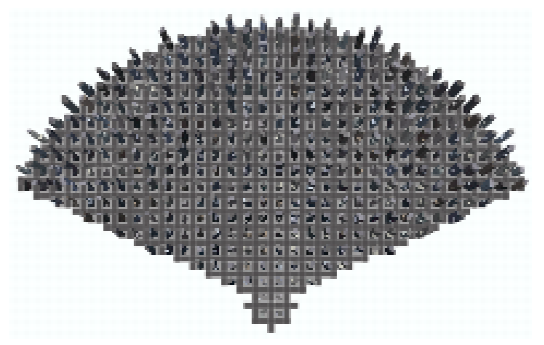
\includegraphics[width=0.85\textwidth]{img/Real-Time-procedural-generation/viewing-range.png}
	\caption{Viewing Range}
	\label{fig:viewingRange}
\end{figure}

\subsubsection{Road Network} % (fold)
\label{ssub:road_network}

The system uses a 2D grid that divide the terrain into square cells. The cells represent proxies for the content that will be procedurally generated. Before the content of each cell is generated, the potential visibility of it is tested, and after that, only the visible cells are filled with content.

Then the roads are created in a uniform grid pattern. This grid does not feel very natural, and in the continuation of the work, this system evolved into a more realistic one with the join of some of the grids to create a less uniform distribution of the buildings.

% subsubsection road_network (end)

\subsubsection{Buildings} % (fold)
\label{ssub:buildings}


To compute the form and appearance of each building, it is used a ``single 32 bit pseudo random number generator seed. The random sequence determines building properties such as width, height and number of floors."
Similar sequences of number result in similar buildings. To avoid that, it is used a a hash function to convert each cell position into a seed.

To generate a building the first is to generate a floor plan. To do so, it is randomly selected and merged a set of regular polygons and rectangles, then this is extruded. This is an iterative process, that creates sections from the top to the bottom, by adding more shapes to the the initial shape and extruding as shown in the Figure~\ref{fig:UC_buildings}. Starting from the left, first there is a simple polygon, that is merged with a rectangle and after extrusion, forms the first block that will be the top of the building. After that, another extrusion is made to generate the next block followed by the merge of a rectangle to the floor shape and the generation of a new block and so on.

\begin{figure}[htbp]
	\centering
	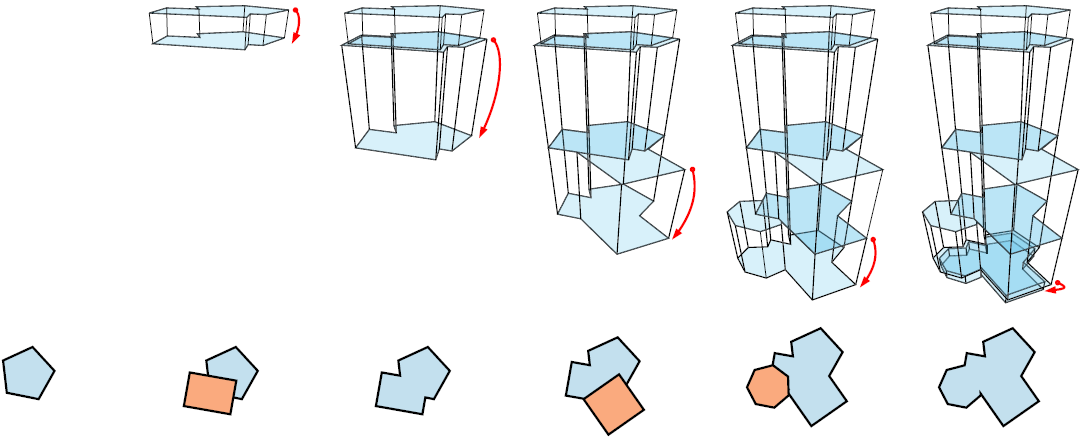
\includegraphics[width=0.85\textwidth]{img/Real-Time-procedural-generation/Building-Generation.png}
	\caption{buildings}
	\label{fig:UC_buildings}
\end{figure}

With the application of this method very complex architectural forms can be generated, depending only on which forms are selected and the order that is used to merge them.

% subsubsection buildings (end)

% subsection undiscovered_city (end)

\subsection{Conclusion} % (fold)
\label{sub:conclusion}

This works present ways to generate and visualize large amounts of geometry, in this cases applied to urban models. While the first \cite{Parish2001} aims to allow the users to create large and realistic urban models, where they give, in the limit, total control to the users, the second one\cite{Greuter2003} is much more a visualization tool, it generates the model automatically for the user to explore.
From this works there are some ideas to explore. The idea of immediate feedback that is implemented in CityEngine, with sliders, is a good input to my work. This helps the unexperienced users to easily know how the users are 

% subsection conclusion (end)


%!TEX root = ../report.tex

%
% Architecture
%

\section{Architecture} % (fold)
\label{sec:architecture}

This work will follow the architecture described in Figure~\ref{fig:architecture}.
There will be a module in Racket that will provide a Racket interface for the rest of the system using \emph{Racket FFI} and is through this that the users will mostly interact with the system. This will be a layer that will not have an impact on performance. 


\begin{wrapfigure}{r}{0.5\textwidth}
	\vspace{-15pt}
    \centering
	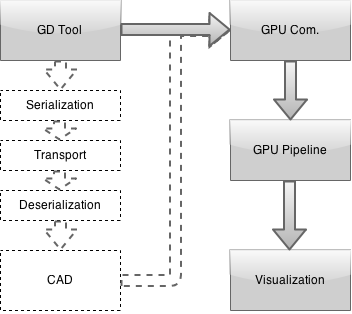
\includegraphics[width=0.5\textwidth]{img/Architecture/GD-Fast-Pipeline.png}
	\caption{High Level Architecture}
	\label{fig:architecture}
	\vspace{-15pt}
\end{wrapfigure}

The second step is the OpenGL layer, that implement the Racket interface and than create the window and manage user input. The functions provided to Racket will create here the description of the geometry that will be \emph{amplified} in the next phase. This description is one $GL\_POINT$ per geometric primitive that represent the position of that primitive and it is also embedded with an array of floats that encode the type of geometry and specific information like size or number of sides.

In the last step are the shaders, where most of the work is done. This receives the small description of the geometry and generates the primitives to be drawn. To achieve this, it is applied the concept of geometry amplification. As told in Section~\ref{sub:geometriy_shaders}, this method has limitations that could make an impact on how the geometry generation is implemented. However OpenGL guarantee support for at least 256 vertices which is enough to generate the majority of geometric primitives. Since this problem is hardware dependent and GPU hardware are getting more powerful I believe that this will not be a problem in the near future.

This architecture significantly reduces the amount of data that is moved between layers and takes advantage of the power that recent GPUs have.

For instance the following code results in the Figure~\ref{fig:pic1} that is a procedural generated model of a city with ~40k buildings. This example was generated with the current prototype with the following Racket code:

\begin{lstlisting}[frame=single,language=Lisp]
(init 0)
(city 100)
(start)
\end{lstlisting}

The \emph{init} command makes an initialization of the system, the \emph{start} command starts creates the window and starts the visualization. In between the model is created, in this case with the function city.

\begin{figure}[htb]
	\centering
	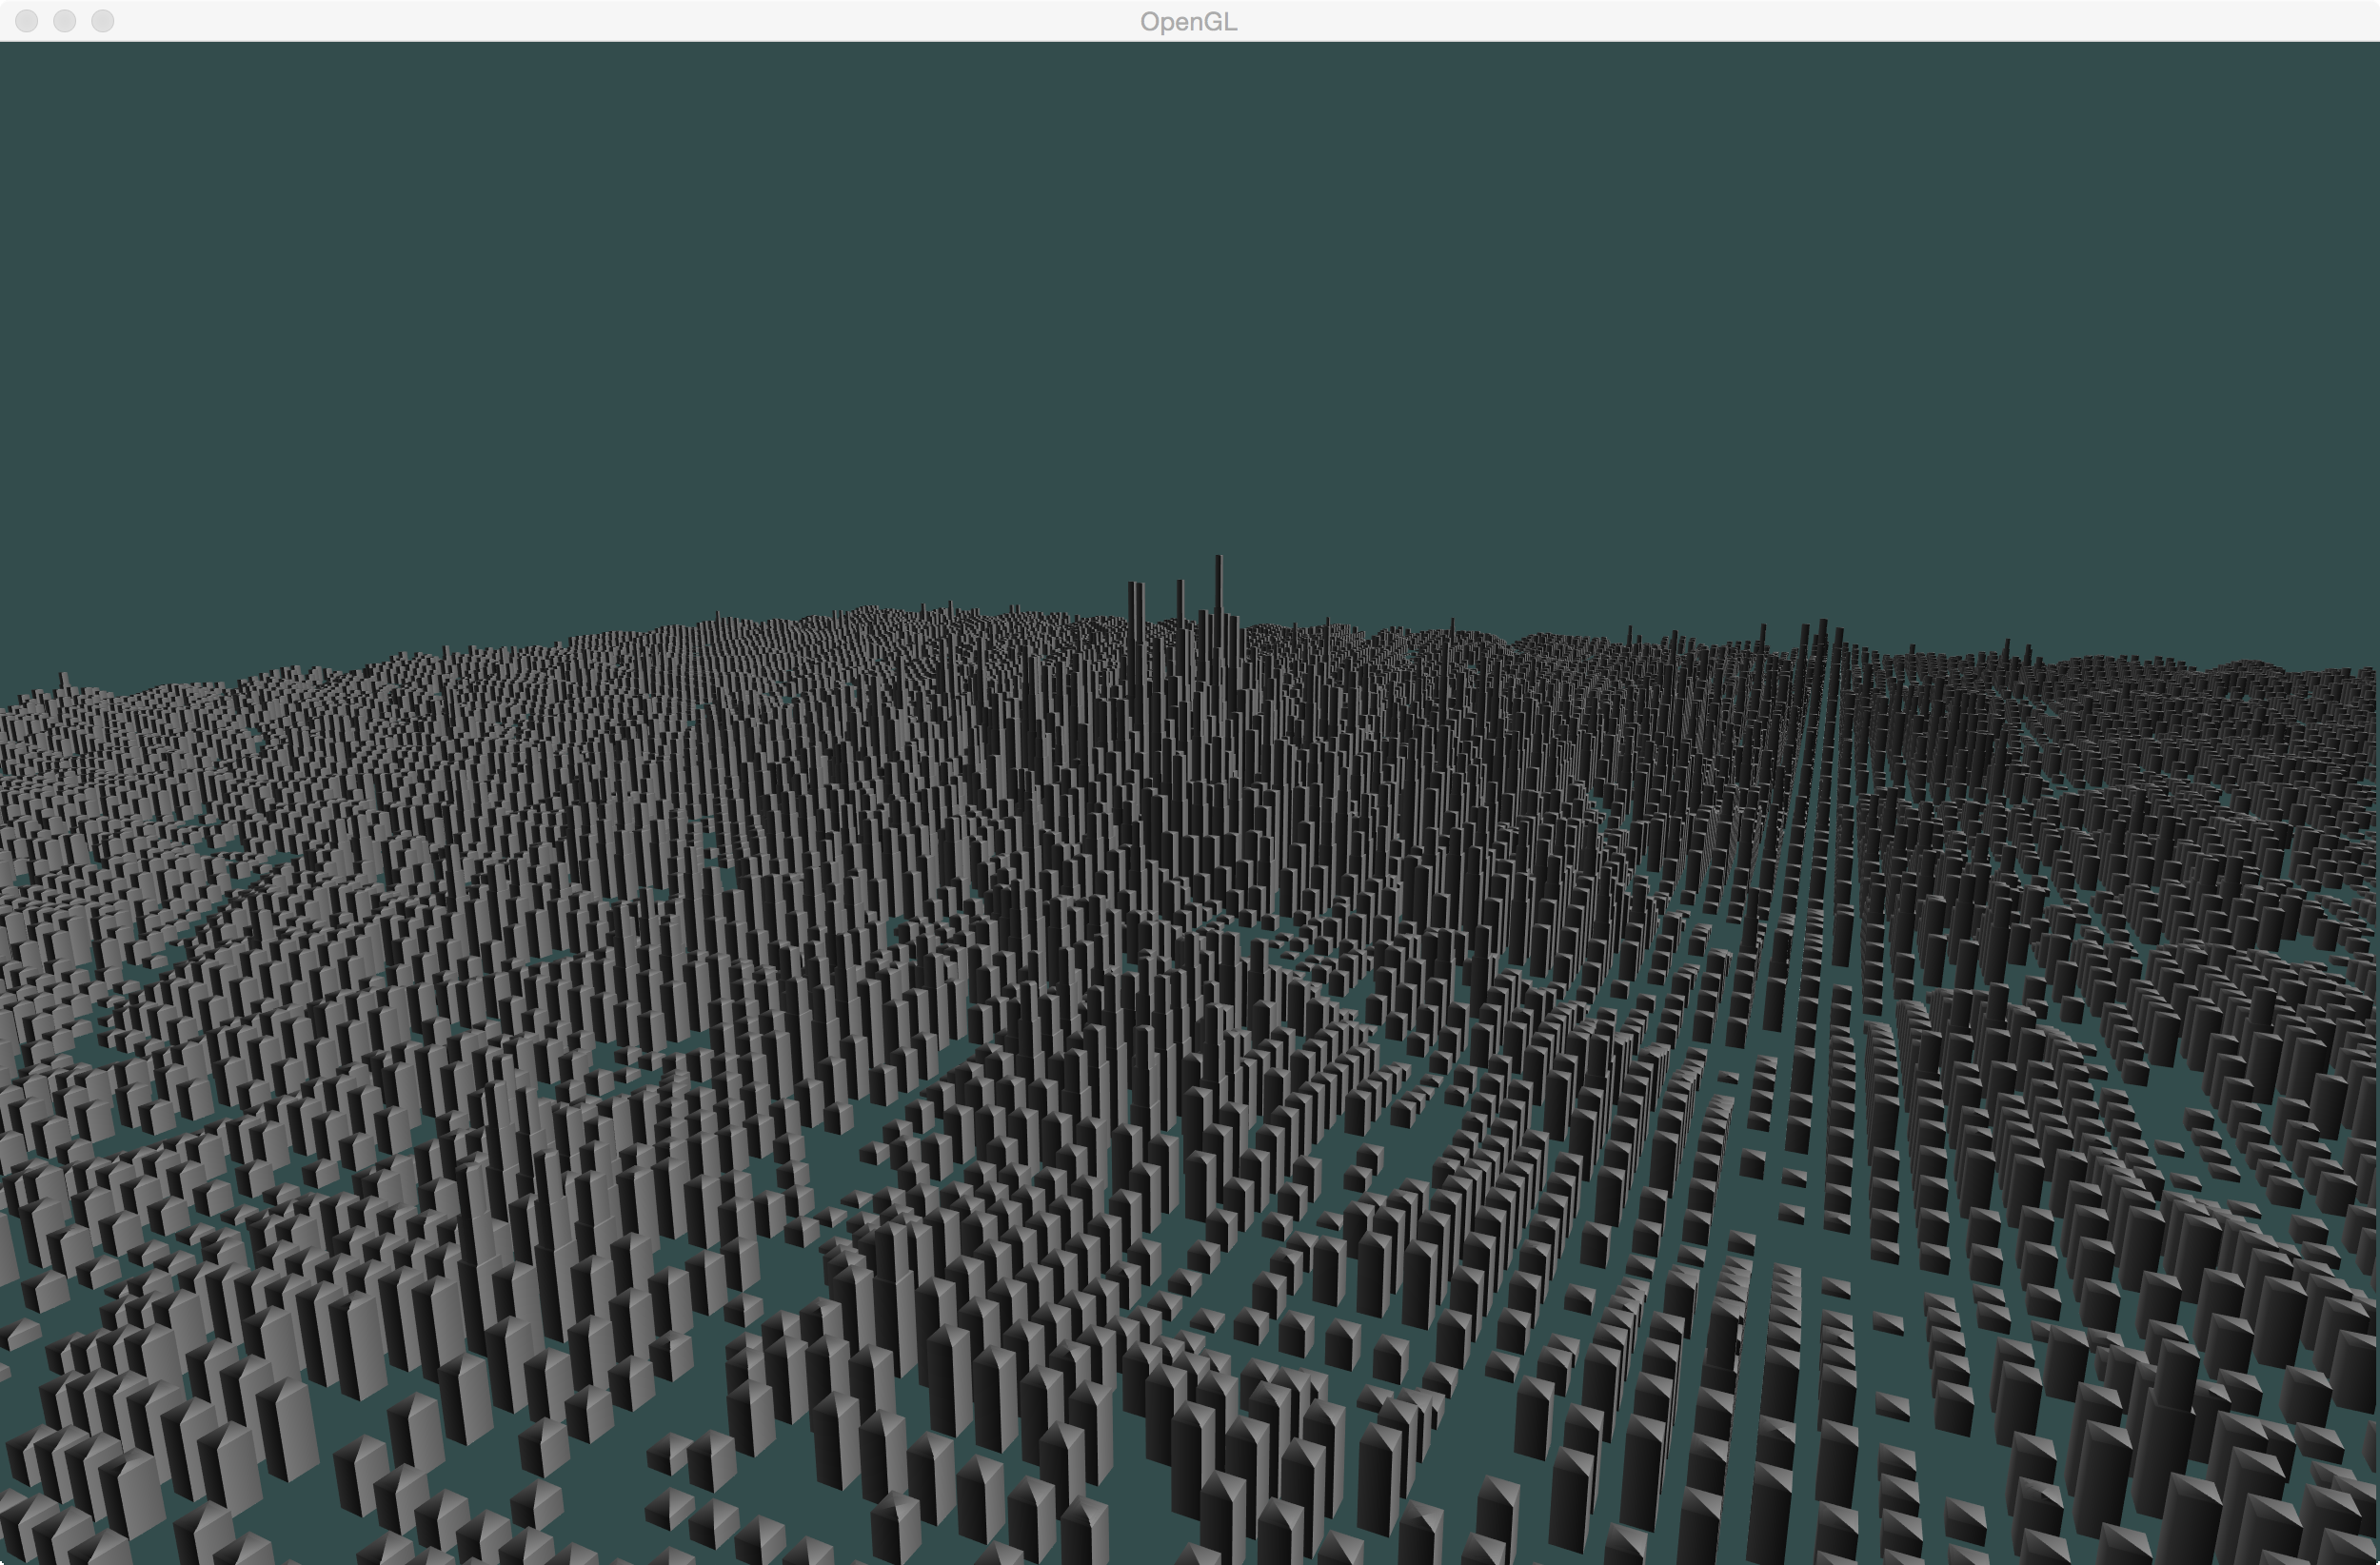
\includegraphics[width=0.95\textwidth]{img/Solution/City2-100*100.png}
	\caption{City Example}
	\label{fig:pic1}
\end{figure}



% section architecture (end)

%!TEX root = ../report.tex

% 
% Evaluation
% 

\section{Evaluation}
\label{sec:evaluation}

This work will be evaluated in two distinct concerns: \emph{functionality} and \emph{performance}.

To evaluate this system will be implemented an interface in Racket to be tested in the context of Rosetta. Rosetta is a GD tool that is largely used by a community of architects that use it to create large models. They have a large amount of examples to be run for comparison. I will use this same set of examples to benchmark my system.

This benchmark will show how broad is the system functionality, and it should implement a large set of functionality that allows the generation of a significant set of the examples. It will also test the correctness of the system, by allowing the comparison and to check if the examples generate the exactly matching results.

And performance is the main concern throughout all this work, and it will be evaluated by comparison with Rosetta's several backends with the same benchmarks.


%Explain how you are going to show your results (statistical data, cpu performance etc). Answer the following questions:
%\begin{itemize}
%  \item Why is this solution going to be better than others.
%  \item How am I going to defend that it is better.
%\end{itemize}
%!TEX root = ../report.tex

% 
% Conclusions
% 

\section{Conclusions}
\label{sec:conclusions}

Architects and designers increasingly use programming as a tool which helps them to develop their work. This powerful tool enables them to create faster and with greater creative freedom. With the development of their programming capabilities they begin to create larger, more complex models and to test the technology at maximum and thus realize their limitations.

The problem of performance arises because the systems being used were not built with this problem in mind. These were developed for a manual, slow usage. It was not thought at the time that a user could generate massive amounts of geometry in seconds. As a result users have to wait for large periods of time since they run their programs until they can see a result.

Therefore there is a need to solve this problem, therefore this work is also needed given that proposes a solution that puts limits on another level allowing users to create.

This solution must have a good performance and support the most used functions that the users need to become a valid alternative to the currently used tools.

My solution shortcuts the Rosetta traditional pipeline to improve performance, doing that by using Rosetta just as an interface and transferring as most of the processing as possible to the GPU.

One prototype is implemented that already creates boxes and cylinders without transformations that allows the creation of the city example in Figure~\ref{fig:pic1}.

In the future, I will explore how to implement the rest of the primitives without losses in performance and how to introduce rotation to the objects without adding much data to the current primitive description set.
%\newpage
%\appendix
%%!TEX root = ../report.tex

\section{Appendix} % (fold)
\label{sec:attachments}

\subsection{Work Scheduling Example} % (fold)
\label{sub:work_scheduling}
\begin{table}[H]
  \caption{Agendamento de trabalho}
  \label{sub:work_scheduling}
  \label{tab:worktable}
  \begin{center}
    \begin{tabular}{|l||c|c|c|c|c|c|c|}
    \hline
       & \textbf{Mai} & \textbf{Jun} & \textbf{Jul} & \textbf{Ago} & \textbf{Out} & \textbf{Nov} & \textbf{Dez}\\
    \hline
    \hline
      Estado da Arte & \cellcolor{black!25} & \cellcolor{black!25} &   &   &   &  &  \\
    \hline
      Desenvolvimento da Solução & \cellcolor{black!25} & \cellcolor{black!25} &   &   &   &   &  \\
    \hline
      Implementação &  & \cellcolor{black!25} & \cellcolor{black!25} & \cellcolor{black!25} &   &   &  \\
    \hline
      Teste e Avaliação &  &  &   & \cellcolor{black!25} & \cellcolor{black!25} &   &  \\
    \hline
      Escrita da Tese & \cellcolor{black!25} & \cellcolor{black!25} & \cellcolor{black!25} & \cellcolor{black!25}  & \cellcolor{black!25} & \cellcolor{black!25} & \cellcolor{black!25} \\
    \hline
      Revisão da Tese &  &  &   &   &  & \cellcolor{black!25} & \cellcolor{black!25} \\
    \hline
    \end{tabular}
  \end{center}
\end{table}



% 
% Bibliography
% 
\bibliographystyle{plain} 

% replace example.bib with your .bib
\bibliography{example.bib} 

\end{document}